% ============================================================
% FEE3411 Control Systems A -- Lecture notes, Week 04
% Topic: Block diagrams and signal flow graphs
%
% Build:  latexmk -pdf week-04-notes.tex
% Needs:  ../tex/preamble.tex (this file lives in Notes/).
% ============================================================
\documentclass[11pt,a4paper]{article}
\usepackage[margin=25mm]{geometry}
% ============================================================
% FEE3411 Control Systems A -- shared preamble
% Used by both the lecture notes (article) and the slides (beamer).
% ============================================================
\usepackage[T1]{fontenc}
% lmodern gives cleaner PDF fonts but is absent from minimal TeX installs.
% Load it only if present, so this preamble builds anywhere.
\IfFileExists{lmodern.sty}{\usepackage{lmodern}}{}
\usepackage{amsmath,amssymb,amsthm}
\usepackage{graphicx}
\usepackage{booktabs}
\usepackage{siunitx}
\usepackage{tikz}
\usepackage{circuitikz}
\usepackage{pgfplots}
\pgfplotsset{compat=1.18}
\usetikzlibrary{arrows.meta,positioning,calc,decorations.markings,shapes.geometric}
\usepackage[most]{tcolorbox}
\usepackage{xcolor}

% ---- Course colours -------------------------------------------------
\definecolor{fnavy}{HTML}{1F3864}
\definecolor{faccent}{HTML}{2E5E4E}
\definecolor{fflag}{HTML}{9C4221}

% ---- Block-diagram style --------------------------------------------
\tikzset{
  block/.style   = {draw, thick, rectangle, minimum height=2.6em,
                    minimum width=3.2em, align=center},
  sumnode/.style = {draw, thick, circle, inner sep=0pt, minimum size=1.6em},
  pickoff/.style = {fill, circle, inner sep=0pt, minimum size=3pt},
  sig/.style     = {-{Latex[length=2mm]}, thick},
}

% ---- Summing-junction signs -----------------------------------------
% \sumsign{<node>}{<angle>}{<+ or ->} places a sign just outside the circle.
\newcommand{\sumsign}[3]{\node[font=\small] at ($(#1)+(#2:0.5)$) {$#3$};}

% ---- Boxed environments ---------------------------------------------
\newtcolorbox{keyidea}[1][]{colback=fnavy!5,colframe=fnavy,
  fonttitle=\bfseries,title=Key idea,#1}
\newtcolorbox{workedex}[1][]{colback=faccent!5,colframe=faccent,
  fonttitle=\bfseries,title=Worked example,#1}
\newtcolorbox{pitfall}[1][]{colback=fflag!5,colframe=fflag,
  fonttitle=\bfseries,title=Common pitfall,#1}

% ---- Shorthands ------------------------------------------------------
\newcommand{\Lap}{\mathcal{L}}
\newcommand{\jw}{\mathrm{j}\omega}
\newcommand{\wn}{\omega_{n}}
\newcommand{\zt}{\zeta}
\newcommand{\TF}[1]{#1(s)}

% ---- Week title machinery -------------------------------------------
\usepackage{fancyhdr}
\newcommand{\thecoursecode}{FEE3411}
\newcommand{\thecoursename}{Control Systems A}
\newcommand{\wknum}{}
\newcommand{\wktopic}{}
\newcommand{\weeknumber}[1]{\renewcommand{\wknum}{#1}}
\newcommand{\weektopic}[1]{\renewcommand{\wktopic}{#1}}
\newcommand{\weektitle}{%
  \thispagestyle{plain}%
  \begin{center}
    {\large\sffamily\bfseries\color{fnavy}\thecoursecode: \thecoursename}\\[2pt]
    {\Huge\sffamily\bfseries Week \wknum}\\[4pt]
    {\LARGE\sffamily\color{fnavy}\wktopic}\\[6pt]
    \rule{\textwidth}{1.2pt}
  \end{center}\vspace{4pt}%
  \pagestyle{fancy}\fancyhf{}%
  \fancyhead[L]{\footnotesize\color{gray}\thecoursecode\ Week \wknum\ --- \wktopic}%
  \fancyhead[R]{\footnotesize\color{gray}\thepage}%
  \renewcommand{\headrulewidth}{0.4pt}%
}

% ---- Outcomes and reading boxes -------------------------------------
\newenvironment{outcomes}
  {\begin{tcolorbox}[colback=white,colframe=fnavy!60,
      fonttitle=\bfseries,title=By the end of this week you should be able to]
   \begin{itemize}[leftmargin=*]}
  {\end{itemize}\end{tcolorbox}}

\newtcolorbox{readingbox}{colback=gray!5,colframe=gray!50,
  fonttitle=\bfseries,title=Reading}

% enumitem must NOT be loaded under beamer: it overwrites beamer's itemize
% templates and the bullet markers silently disappear. The notes (article) get
% it; the slides (beamer) use beamer's own list machinery instead.
\makeatletter
\@ifclassloaded{beamer}{}{\usepackage{enumitem}}
\makeatother


% The shared preamble's \sumsign places a sign at radius 0.5 in \small, which
% is too close to the circle for these diagrams -- the sign merges with the
% incoming arrowhead. Push it out and shrink it, for this file only. Signs are
% then placed 30 degrees off the arrow they belong to, never on it.
\renewcommand{\sumsign}[3]{\node[font=\scriptsize] at ($(#1)+(#2:0.72)$) {$#3$};}

\weeknumber{4}
\weektopic{Block Diagrams and Signal Flow Graphs}

\begin{document}
\weektitle

% --------------------------------------------------------------------
\section*{What this week covers}

\begin{outcomes}
\item Draw the block diagram of an interconnected system, using the three
      elements --- block, summing junction and pick-off point --- and state the
      no-loading assumption that the cascade rule depends on.
\item Reduce the three basic connections (cascade, parallel, feedback) to a
      single block, deriving the closed-loop formula rather than quoting it.
\item Identify, for a system in canonical feedback form, the forward-path,
      open-loop, closed-loop and error transfer functions, and write down the
      characteristic equation.
\item Apply the rules of block-diagram algebra --- including moving a summing
      junction or a pick-off point past a block --- to reduce a multi-loop
      diagram to one transfer function.
\item Convert a block diagram to a signal flow graph, and identify its forward
      paths, loops, loop gains and non-touching loops.
\item Evaluate a transfer function with Mason's gain formula, including the
      non-touching-loop terms of $\Delta$ and the cofactors $\Delta_k$, and
      check the result against block-diagram reduction.
\item Find the response of a system with more than one input by superposition,
      computing one transfer function per input.
\end{outcomes}

\begin{readingbox}
\textbf{Primary} --- Khalil, \S2-3 Block Diagrams (pp.~40--49).\\
\textbf{Secondary} --- Nise (6th ed.), \S5.2 Block Diagrams (p.~236); \S5.3
Analysis and Design of Feedback Systems (p.~245); \S5.4 Signal-Flow Graphs
(p.~248); \S5.5 Mason's Rule (p.~251). \emph{Khalil does not cover signal flow
graphs --- for \S\ref{sec:sfg}--\S\ref{sec:mason} Nise is the primary text.}\\
\textbf{Further} --- Nagrath \& Gopal (2nd ed.), \S2.4 Block Diagram Algebra
(p.~38), \S2.5 Signal Flow Graphs (p.~45); Sundararajan, \S5.1, \S5.2,
\S5.2.1.
\end{readingbox}

\noindent
\emph{Contact hours this week:} 2\,h lecture $+$ 1\,h tutorial.\\
\emph{Syllabus items addressed:} ``Block diagrams and canonical feedback.
Derivation of transfer functions from the reduction of elementary block
diagrams. Construction of signal flow diagrams. Block diagram reduction using
signal flow diagrams.'' (Transfer Functions); ``Block diagrams'' (Time Domain
Linear Systems Analysis).\\
\emph{Expected learning outcomes:} ELO~2 --- \emph{analyse a control system
solution in the time- and frequency-domains}; ELO~1 --- \emph{describe the
working principles of a given control system} (the block diagram is how a
control system's working principle is described on paper).

\bigskip
\noindent
\textbf{A note on the two halves.} The first hour is block diagrams: the
elements, the three basic connections, the canonical feedback form, and the
algebra for reducing a multi-loop diagram by hand. That algebra works, but it
gets awkward as soon as two loops overlap, and \S\ref{sec:overlap} shows exactly
where it starts to hurt. The second hour answers that with signal flow graphs
and Mason's gain formula, which read the same answer off the same diagram
without redrawing it once. Week~3 gave us the transfer function of a single
component; this week is about what happens when components are wired together,
which is the last piece of machinery needed before Week~5 starts asking how
these systems actually respond.

% ====================================================================
\part*{Part A --- Block diagrams}
\addcontentsline{toc}{part}{Part A}

% --------------------------------------------------------------------
\section{From one block to many}
\label{sec:elements}

Week~3 produced transfer functions for single components: a network, a motor, a
mass on a spring. A real control system is several of these wired together ---
a reference input compared against a measurement, the difference amplified,
the amplifier driving a motor, the motor's shaft position measured by a sensor
that closes the loop. To get the transfer function of the whole thing we need a
notation for the wiring, and rules for collapsing it.

A \textbf{block diagram} is that notation. It has exactly three elements, shown
in Figure~\ref{fig:elements}.

\begin{figure}[htbp]
\centering
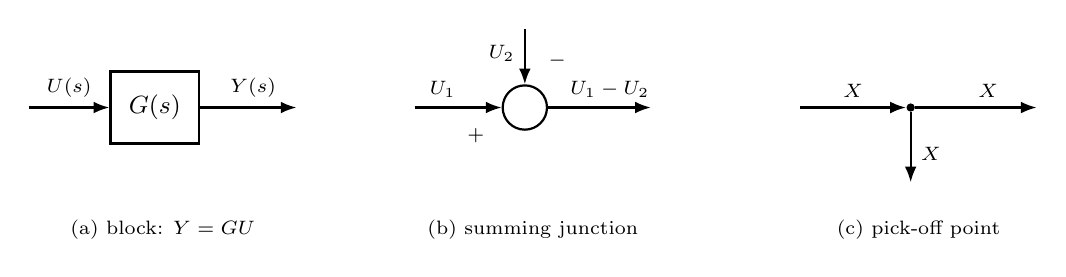
\begin{tikzpicture}[x=1cm,y=1cm,font=\small]
% ---------- (a) block ----------
\begin{scope}[shift={(0,0)}]
\node[block] (G) at (1.7,0) {$G(s)$};
\draw[sig] (0.1,0) -- node[above,font=\scriptsize]{$U(s)$} (G);
\draw[sig] (G) -- (3.5,0) node[above,font=\scriptsize,pos=0.55]{$Y(s)$};
\node[font=\scriptsize,align=center] at (1.8,-1.55)
  {(a) block: $Y=GU$};
\end{scope}
% ---------- (b) summing junction ----------
\begin{scope}[shift={(4.9,0)}]
\node[sumnode] (S) at (1.5,0) {};
\draw[sig] (0.1,0) -- node[above,font=\scriptsize,pos=0.32]{$U_1$} (S);
\draw[sig] (1.5,1.0) -- node[left,font=\scriptsize,pos=0.45]{$U_2$} (S);
\draw[sig] (S) -- (3.1,0) node[above,font=\scriptsize,pos=0.6]{$U_1-U_2$};
\sumsign{S}{210}{+}
\sumsign{S}{55}{-}
\node[font=\scriptsize,align=center] at (1.6,-1.55)
  {(b) summing junction};
\end{scope}
% ---------- (c) pick-off point ----------
\begin{scope}[shift={(9.8,0)}]
\node[pickoff] (P) at (1.5,0) {};
\draw[sig] (0.1,0) -- node[above,font=\scriptsize]{$X$} (P);
\draw[sig] (P) -- (3.1,0) node[above,font=\scriptsize,pos=0.6]{$X$};
\draw[sig] (P) -- (1.5,-0.95) node[right,font=\scriptsize,pos=0.6]{$X$};
\node[font=\scriptsize,align=center] at (1.6,-1.55)
  {(c) pick-off point};
\end{scope}
\end{tikzpicture}
\caption{The three elements of a block diagram. A block multiplies its input
by a transfer function; a summing junction adds signals with the signs marked
beside it; a pick-off point sends the \emph{same} signal down two branches.
Cf.\ Khalil Figs.~2-31 and 2-32, pp.~40--41.}
\label{fig:elements}
\end{figure}

Two things about this notation matter more than they first appear.

First, \textbf{a pick-off point does not divide the signal.} Both branches
carry $X$ in full. This is the opposite of a wire junction in a circuit, where
current divides; the block diagram is a diagram of \emph{signals}, not of power
flow, and taking a copy of a signal costs nothing.

Second, and more consequentially: writing two blocks in cascade and multiplying
their transfer functions assumes the second does not \emph{load} the first.

\begin{pitfall}
Cascading $G_1$ and $G_2$ to get $G_1G_2$ assumes that connecting $G_2$ does
not change $G_1$'s output --- that is, that $G_2$ draws no current (or torque,
or flow) from $G_1$. Two $RC$ networks in series are the standard trap: each
alone has transfer function $1/(RCs+1)$, but wired directly together their
combined transfer function is \emph{not} $1/(RCs+1)^2$, because the second
network's input impedance loads the first. Cascade blocks only where a buffer
amplifier separates the stages, or where the impedances make loading
negligible --- and if a question gives you a circuit rather than a diagram, go
back to the impedance method of Week~3 and derive the whole thing at once.
\end{pitfall}

\begin{keyidea}
A block diagram is a picture of a set of simultaneous algebraic equations in
$s$ --- one equation per block and per summing junction. Every reduction rule
in this week's work is nothing more than eliminating an internal variable
between those equations. If a diagram ever defeats you, write its equations out
and solve them; you will always get the right answer, just more slowly.
\end{keyidea}

% --------------------------------------------------------------------
\section{The three basic connections}
\label{sec:connections}

Every block diagram, however tangled, is built from three connections:
cascade, parallel and feedback. Figure~\ref{fig:three} shows each with its
single-block equivalent.

\begin{figure}[htbp]
\centering
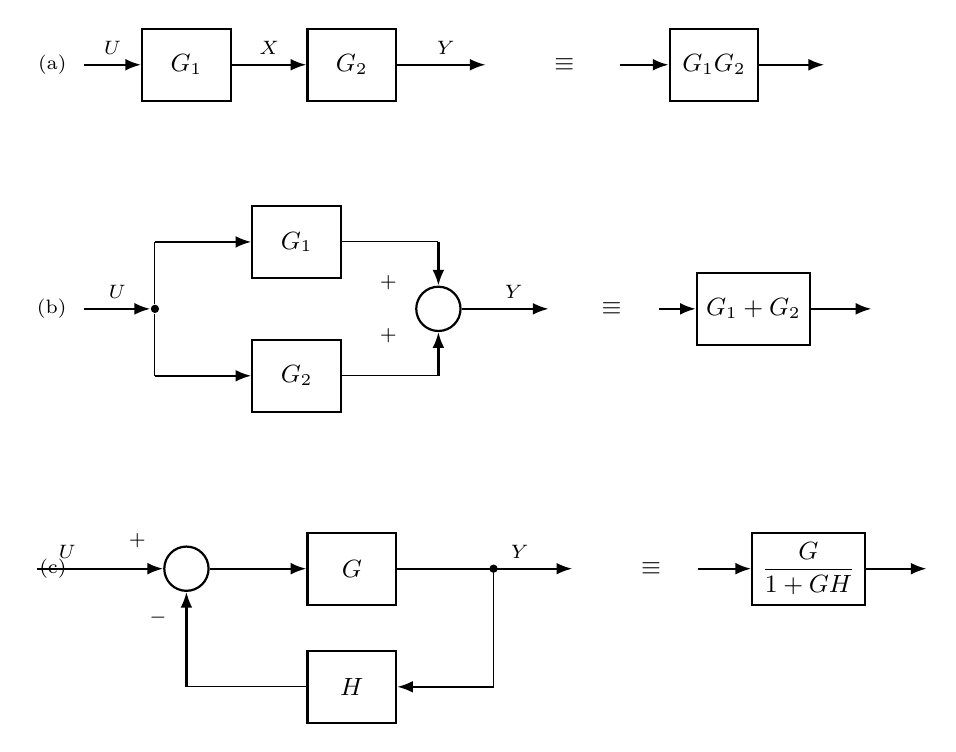
\begin{tikzpicture}[x=1cm,y=1cm,font=\small]
% ---------- (a) cascade ----------
\begin{scope}[shift={(0,0)}]
\node[block] (A1) at (1.5,0) {$G_1$};
\node[block] (A2) at (3.6,0) {$G_2$};
\draw[sig] (0.2,0) -- node[above,font=\scriptsize]{$U$} (A1);
\draw[sig] (A1) -- node[above,font=\scriptsize]{$X$} (A2);
\draw[sig] (A2) -- (5.3,0) node[above,font=\scriptsize,pos=0.55]{$Y$};
\node at (6.3,0) {$\equiv$};
\node[block] (A3) at (8.2,0) {$G_1G_2$};
\draw[sig] (7.0,0) -- (A3);
\draw[sig] (A3) -- (9.6,0);
\node[font=\scriptsize,left] at (0.1,0) {(a)};
\end{scope}
% ---------- (b) parallel ----------
\begin{scope}[shift={(0,-3.1)}]
\node[pickoff] (P) at (1.1,0) {};
\node[block] (B1) at (2.9,0.85) {$G_1$};
\node[block] (B2) at (2.9,-0.85) {$G_2$};
\node[sumnode] (SB) at (4.7,0) {};
\draw[sig] (0.2,0) -- node[above,font=\scriptsize]{$U$} (P);
\draw (P) -- (1.1,0.85); \draw[sig] (1.1,0.85) -- (B1);
\draw (P) -- (1.1,-0.85); \draw[sig] (1.1,-0.85) -- (B2);
\draw (B1) -- (4.7,0.85); \draw[sig] (4.7,0.85) -- (SB);
\draw (B2) -- (4.7,-0.85); \draw[sig] (4.7,-0.85) -- (SB);
\sumsign{SB}{152}{+}
\sumsign{SB}{208}{+}
\draw[sig] (SB) -- (6.1,0) node[above,font=\scriptsize,pos=0.6]{$Y$};
\node at (6.9,0) {$\equiv$};
\node[block] (B3) at (8.7,0) {$G_1+G_2$};
\draw[sig] (7.5,0) -- (B3);
\draw[sig] (B3) -- (10.2,0);
\node[font=\scriptsize,left] at (0.1,0) {(b)};
\end{scope}
% ---------- (c) feedback ----------
\begin{scope}[shift={(0,-6.4)}]
\node[sumnode] (SC) at (1.5,0) {};
\node[block] (C1) at (3.6,0) {$G$};
\node[pickoff] (PC) at (5.4,0) {};
\node[block] (C2) at (3.6,-1.5) {$H$};
\draw[sig] (-0.4,0) -- node[above,font=\scriptsize,pos=0.24]{$U$} (SC);
\draw[sig] (SC) -- (C1);
\draw[sig] (C1) -- (6.4,0) node[above,font=\scriptsize,pos=0.7]{$Y$};
\draw (PC) -- (5.4,-1.5); \draw[sig] (5.4,-1.5) -- (C2);
\draw (C2) -- (1.5,-1.5); \draw[sig] (1.5,-1.5) -- (SC);
\sumsign{SC}{150}{+}
\sumsign{SC}{240}{-}
\node at (7.4,0) {$\equiv$};
\node[block] (C3) at (9.4,0) {$\dfrac{G}{1+GH}$};
\draw[sig] (8.0,0) -- (C3);
\draw[sig] (C3) -- (10.9,0);
\node[font=\scriptsize,left] at (0.1,0) {(c)};
\end{scope}
\end{tikzpicture}
\caption{The three basic connections and their single-block equivalents:
(a) cascade, (b) parallel, (c) negative feedback. Cf.\ Khalil Fig.~2-34,
p.~41; Nise \S5.2, pp.~236--240.}
\label{fig:three}
\end{figure}

\paragraph{Cascade.} With $X=G_1U$ and $Y=G_2X$, substitution gives
$Y=G_2G_1U$, so the equivalent transfer function is the \emph{product}
$G_1G_2$. Order does not matter algebraically, because transfer functions are
scalar rational functions and multiplication commutes --- which is worth
noticing, because the physical systems certainly do not commute. Swapping a
real amplifier and a real motor would matter; swapping their transfer functions
does not.

\paragraph{Parallel.} With both blocks fed the same $U$ from a pick-off point
and their outputs summed, $Y=G_1U\pm G_2U$, so the equivalent is
$G_1\pm G_2$ --- a \emph{sum}, with whatever signs the summing junction
carries.

\paragraph{Feedback.} This one deserves the full derivation, because it is the
formula the rest of the unit runs on. Let the summing junction subtract the
feedback signal, so that with $E$ the signal at the junction's output,
\[
  E = U - HY, \qquad Y = GE .
\]
Eliminating $E$ between the two,
\[
  Y = G\left(U - HY\right)
  \quad\Longrightarrow\quad
  Y\left(1 + GH\right) = GU
  \quad\Longrightarrow\quad
  \boxed{\;\frac{Y}{U} = \frac{G}{1+GH}\;}.
\]
If the junction \emph{adds} the feedback signal instead --- positive feedback
--- the same two lines give $G/(1-GH)$. The sign in the denominator is
therefore the opposite of the sign at the summing junction, which is the single
most common place to lose a minus sign in this entire unit.

\begin{pitfall}
Read the sign off the \emph{diagram}, not off memory. The formula
$G/(1+GH)$ is for negative feedback, where the junction subtracts. A diagram
with a $+$ at the feedback input needs $G/(1-GH)$, and that system is a
completely different animal: its denominator can vanish, which is exactly what
instability looks like. When a question's answer comes out with a suspicious
sign, check the summing junction first.
\end{pitfall}

% --------------------------------------------------------------------
\section{The canonical feedback form}
\label{sec:canonical}

Almost every control system in this unit is drawn, eventually, in the form of
Figure~\ref{fig:canonical}: a reference in, a comparison, a forward path, a
measurement path back. It is worth having names for its parts, because
examination questions and textbooks both use them freely.

\begin{figure}[htbp]
\centering
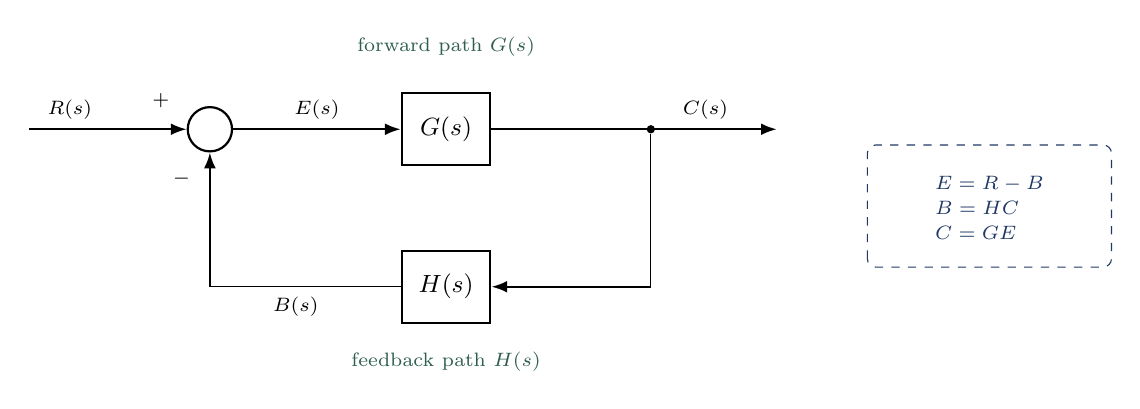
\begin{tikzpicture}[x=1cm,y=1cm,font=\small]
\node[sumnode] (S) at (2.0,0) {};
\node[block] (G) at (5.0,0) {$G(s)$};
\node[pickoff] (P) at (7.6,0) {};
\node[block] (H) at (5.0,-2.0) {$H(s)$};
\draw[sig] (-0.3,0) -- node[above,font=\scriptsize,pos=0.26]{$R(s)$} (S);
\draw[sig] (S) -- node[above,font=\scriptsize]{$E(s)$} (G);
\draw[sig] (G) -- (9.2,0) node[above,font=\scriptsize,pos=0.75]{$C(s)$};
\draw (P) -- (7.6,-2.0); \draw[sig] (7.6,-2.0) -- (H);
\draw (H) -- node[below,font=\scriptsize,pos=0.55]{$B(s)$} (2.0,-2.0);
\draw[sig] (2.0,-2.0) -- (S);
\sumsign{S}{150}{+}
\sumsign{S}{240}{-}
% annotations, all placed clear of the wires
\node[faccent,font=\scriptsize,align=center] at (5.0,1.05) {forward path $G(s)$};
\node[faccent,font=\scriptsize,align=center] at (5.0,-2.95) {feedback path $H(s)$};
\node[fnavy,font=\scriptsize,align=left] at (11.9,-1.0)
  {$E=R-B$\\[1pt] $B=HC$\\[1pt] $C=GE$};
\draw[fnavy,dashed,rounded corners=3pt] (10.35,-1.75) rectangle (13.45,-0.2);
\end{tikzpicture}
\caption{The canonical negative-feedback form, with the three equations it
encodes. $R$ is the reference, $C$ the controlled output, $B$ the feedback
signal and $E$ the actuating error signal. Cf.\ Nagrath \& Gopal Fig.~2.20,
p.~40.}
\label{fig:canonical}
\end{figure}

Eliminating $E$ and $B$ from the three equations beside the figure gives the
four transfer functions that get quoted by name:
\begin{align}
  \text{forward-path (or plant) transfer function:}\quad & G(s) \nonumber\\
  \text{open-loop transfer function (loop gain):}\quad & G(s)H(s) \nonumber\\
  \text{closed-loop transfer function:}\quad & T(s)=\frac{C(s)}{R(s)}
    = \frac{G(s)}{1+G(s)H(s)} \label{eq:closedloop}\\
  \text{error transfer function:}\quad & \frac{E(s)}{R(s)}
    = \frac{1}{1+G(s)H(s)} \label{eq:errortf}
\end{align}
When $H(s)=1$ the system is called \textbf{unity feedback}, the measurement is
taken as perfect, and $E$ becomes the true error $R-C$.

\begin{keyidea}
The denominator of the closed-loop transfer function is $1+G(s)H(s)$, so the
closed-loop poles are the roots of
\[
  1 + G(s)H(s) = 0 ,
\]
the \textbf{characteristic equation} of the closed-loop system. This single
equation is the object of Weeks~7, 8, 11 and 12: Routh--Hurwitz tests whether
its roots are in the left half plane, the root locus tracks where they move as
a gain varies, and the Nyquist criterion counts them from a frequency-response
plot. Everything downstream of this week is about the roots of $1+GH=0$.
\end{keyidea}

\begin{pitfall}
The open-loop transfer function is $G(s)H(s)$, the gain around the whole loop
--- not the forward path $G(s)$ alone, and not the closed-loop $T(s)$ with the
loop cut. The three are equal only in the trivial case $H=1$ and no feedback at
all. When a question says ``for the open-loop transfer function
$G(s)H(s)=K/[s(s+2)]$'', it is handing you the \emph{product}, and the
characteristic equation is $1+K/[s(s+2)]=0$ directly.
\end{pitfall}

\begin{workedex}[breakable, title=Worked example 4.1 --- what feedback does to the poles]
A unity-feedback system has forward path
\[
  G(s)=\frac{8}{s(s+6)},\qquad H(s)=1 .
\]
Find the closed-loop transfer function, its poles, its d.c.\ gain, and the
error transfer function. Compare the closed-loop poles with the open-loop
poles.

\medskip
\textbf{Closed-loop transfer function.} From \eqref{eq:closedloop},
\[
  T(s)=\frac{G}{1+GH}
   =\frac{\dfrac{8}{s(s+6)}}{1+\dfrac{8}{s(s+6)}}
   =\frac{8}{s(s+6)+8}
   =\frac{8}{s^{2}+6s+8}
   =\frac{8}{(s+2)(s+4)} .
\]
The middle step --- multiplying numerator and denominator by $s(s+6)$ --- is
the one worth doing carefully; it is where the $1$ in $1+GH$ turns into the
open-loop denominator.

\medskip
\textbf{Poles.} Open loop, $G$ has poles at $s=0$ and $s=-6$: one of them is
at the origin, so the open-loop system is only marginally stable and its step
response would ramp away without bound. Closed loop, the poles are at $s=-2$
and $s=-4$ --- both strictly in the left half plane. Closing the loop has
moved both poles and made the system stable.

\medskip
\textbf{d.c.\ gain.} $T(0)=8/8=1$. The closed-loop system follows a constant
reference exactly, which is what the free integrator in $G$ buys us --- a
result Week~6 will make precise as ``a type-1 system has zero steady-state
error to a step''.

\medskip
\textbf{Error transfer function.} From \eqref{eq:errortf},
\[
  \frac{E(s)}{R(s)}=\frac{1}{1+GH}=\frac{s(s+6)}{s^{2}+6s+8} ,
\]
whose d.c.\ gain is $0$ --- the same statement as $T(0)=1$, read from the other
side.

\medskip
\textbf{What it means.} Feedback did not add or remove any modes: the
closed-loop system still has two poles, because $1+GH=0$ still has degree two.
What it did was \emph{relocate} them, from $\{0,-6\}$ to $\{-2,-4\}$. That
relocation is the whole point of feedback, and choosing where to put the poles
is what FEE3412 calls design.
\end{workedex}

% --------------------------------------------------------------------
\section{Block-diagram algebra}
\label{sec:algebra}

The three basic connections handle diagrams whose loops are neatly nested. Real
diagrams need a few more moves, collected in Table~\ref{tab:rules}. Each is
proved the same way: write the equations for the signals before and after, and
check they agree.

\begin{table}[htbp]
\centering
\caption{The rules of block-diagram algebra. Each row's two diagrams are
equivalent. Cf.\ Nagrath \& Gopal Table~2.4, p.~42; Nise \S5.2, p.~236.}
\label{tab:rules}
\small
\renewcommand{\arraystretch}{1.2}
\setlength{\tabcolsep}{3pt}
\begin{tabular}{@{}>{\raggedright\arraybackslash}p{2.95cm}@{}c@{\hspace{6mm}}c@{}}
\toprule
\textbf{Rule} & \textbf{Original} & \textbf{Equivalent}\\
\midrule
%
Combine blocks in cascade &
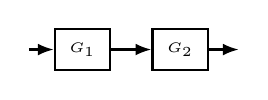
\begin{tikzpicture}[x=0.62cm,y=0.50cm,baseline=(current bounding box.center),font=\tiny]
\node[block,minimum height=1.5em,minimum width=2em] (a) at (1.1,0) {$G_1$};
\node[block,minimum height=1.5em,minimum width=2em] (b) at (3.1,0) {$G_2$};
\draw[sig] (0,0) -- (a); \draw[sig] (a) -- (b); \draw[sig] (b) -- (4.3,0);
\end{tikzpicture} &
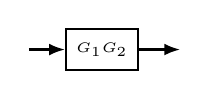
\begin{tikzpicture}[x=0.62cm,y=0.50cm,baseline=(current bounding box.center),font=\tiny]
\node[block,minimum height=1.5em,minimum width=2.6em] (a) at (1.5,0) {$G_1G_2$};
\draw[sig] (0,0) -- (a); \draw[sig] (a) -- (3.1,0);
\end{tikzpicture}\\[5mm]
%
Combine blocks in parallel &
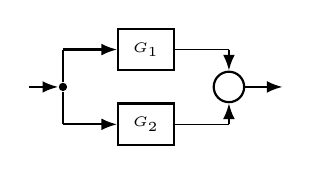
\begin{tikzpicture}[x=0.62cm,y=0.50cm,baseline=(current bounding box.center),font=\tiny]
\node[pickoff] (p) at (0.7,0) {};
\node[block,minimum height=1.5em,minimum width=2em] (a) at (2.4,0.95) {$G_1$};
\node[block,minimum height=1.5em,minimum width=2em] (b) at (2.4,-0.95) {$G_2$};
\node[sumnode,minimum size=1.1em] (s) at (4.1,0) {};
\draw[sig] (0,0) -- (p);
\draw (p) -- (0.7,0.95); \draw[sig] (0.7,0.95) -- (a);
\draw (p) -- (0.7,-0.95); \draw[sig] (0.7,-0.95) -- (b);
\draw (a) -- (4.1,0.95); \draw[sig] (4.1,0.95) -- (s);
\draw (b) -- (4.1,-0.95); \draw[sig] (4.1,-0.95) -- (s);
\draw[sig] (s) -- (5.2,0);
\end{tikzpicture} &
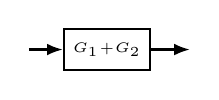
\begin{tikzpicture}[x=0.62cm,y=0.50cm,baseline=(current bounding box.center),font=\tiny]
\node[block,minimum height=1.5em,minimum width=3em] (a) at (1.6,0) {$G_1\!+\!G_2$};
\draw[sig] (0,0) -- (a); \draw[sig] (a) -- (3.3,0);
\end{tikzpicture}\\[5mm]
%
Eliminate a feedback loop &
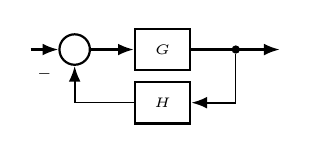
\begin{tikzpicture}[x=0.62cm,y=0.50cm,baseline=(current bounding box.center),font=\tiny]
\node[sumnode,minimum size=1.1em] (s) at (0.9,0) {};
\node[block,minimum height=1.5em,minimum width=2em] (a) at (2.7,0) {$G$};
\node[pickoff] (p) at (4.2,0) {};
\node[block,minimum height=1.5em,minimum width=2em] (h) at (2.7,-1.35) {$H$};
\draw[sig] (0,0) -- (s); \draw[sig] (s) -- (a); \draw[sig] (a) -- (5.1,0);
\draw (p) -- (4.2,-1.35); \draw[sig] (4.2,-1.35) -- (h);
\draw (h) -- (0.9,-1.35); \draw[sig] (0.9,-1.35) -- (s);
\node[font=\tiny] at (0.28,-0.62) {$-$};
\end{tikzpicture} &
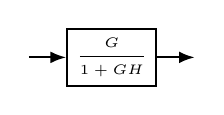
\begin{tikzpicture}[x=0.62cm,y=0.50cm,baseline=(current bounding box.center),font=\tiny]
\node[block,minimum height=1.9em,minimum width=3em] (a) at (1.7,0) {$\dfrac{G}{1+GH}$};
\draw[sig] (0,0) -- (a); \draw[sig] (a) -- (3.4,0);
\end{tikzpicture}\\[5mm]
%
Move a summing junction back through a block &
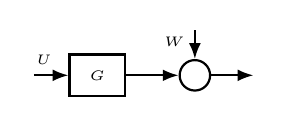
\begin{tikzpicture}[x=0.62cm,y=0.50cm,baseline=(current bounding box.center),font=\tiny]
\node[block,minimum height=1.5em,minimum width=2em] (a) at (1.3,0) {$G$};
\node[sumnode,minimum size=1.1em] (s) at (3.3,0) {};
\draw[sig] (0,0) -- node[above,font=\tiny,pos=0.3]{$U$} (a);
\draw[sig] (a) -- (s); \draw[sig] (s) -- (4.5,0);
\draw[sig] (3.3,1.15) -- node[left,font=\tiny,pos=0.4]{$W$} (s);
\end{tikzpicture} &
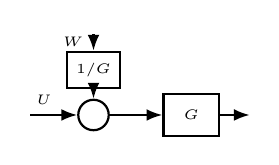
\begin{tikzpicture}[x=0.62cm,y=0.50cm,baseline=(current bounding box.center),font=\tiny]
\node[sumnode,minimum size=1.1em] (s) at (1.3,0) {};
\node[block,minimum height=1.5em,minimum width=2em] (a) at (3.3,0) {$G$};
\draw[sig] (0,0) -- node[above,font=\tiny,pos=0.3]{$U$} (s);
\draw[sig] (s) -- (a); \draw[sig] (a) -- (4.5,0);
\node[block,minimum height=1.3em,minimum width=1.6em] (k) at (1.3,1.15) {$1/G$};
\draw[sig] (1.3,2.05) -- node[left,font=\tiny,pos=0.45]{$W$} (k);
\draw[sig] (k) -- (s);
\end{tikzpicture}\\[5mm]
%
Move a pick-off point forward through a block &
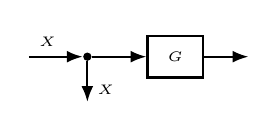
\begin{tikzpicture}[x=0.62cm,y=0.50cm,baseline=(current bounding box.center),font=\tiny]
\node[pickoff] (p) at (1.2,0) {};
\node[block,minimum height=1.5em,minimum width=2em] (a) at (3.0,0) {$G$};
\draw[sig] (0,0) -- node[above,font=\tiny,pos=0.35]{$X$} (p);
\draw[sig] (p) -- (a); \draw[sig] (a) -- (4.5,0);
\draw[sig] (p) -- (1.2,-1.15) node[right,font=\tiny,pos=0.7]{$X$};
\end{tikzpicture} &
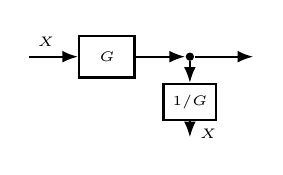
\begin{tikzpicture}[x=0.62cm,y=0.50cm,baseline=(current bounding box.center),font=\tiny]
\node[block,minimum height=1.5em,minimum width=2em] (a) at (1.6,0) {$G$};
\node[pickoff] (p) at (3.3,0) {};
\draw[sig] (0,0) -- node[above,font=\tiny,pos=0.35]{$X$} (a);
\draw[sig] (a) -- (p); \draw[sig] (p) -- (4.6,0);
\node[block,minimum height=1.3em,minimum width=1.6em] (k) at (3.3,-1.15) {$1/G$};
\draw[sig] (p) -- (k);
\draw[sig] (k) -- (3.3,-2.05) node[right,font=\tiny,pos=0.75]{$X$};
\end{tikzpicture}\\[5mm]
%
Interchange adjacent summing junctions &
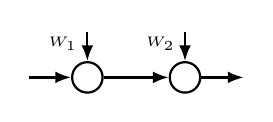
\begin{tikzpicture}[x=0.62cm,y=0.50cm,baseline=(current bounding box.center),font=\tiny]
\node[sumnode,minimum size=1.1em] (s1) at (1.2,0) {};
\node[sumnode,minimum size=1.1em] (s2) at (3.2,0) {};
\draw[sig] (0,0) -- (s1); \draw[sig] (s1) -- (s2); \draw[sig] (s2) -- (4.4,0);
\draw[sig] (1.2,1.15) -- node[left,font=\tiny,pos=0.4]{$W_1$} (s1);
\draw[sig] (3.2,1.15) -- node[left,font=\tiny,pos=0.4]{$W_2$} (s2);
\end{tikzpicture} &
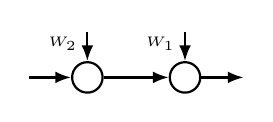
\begin{tikzpicture}[x=0.62cm,y=0.50cm,baseline=(current bounding box.center),font=\tiny]
\node[sumnode,minimum size=1.1em] (s1) at (1.2,0) {};
\node[sumnode,minimum size=1.1em] (s2) at (3.2,0) {};
\draw[sig] (0,0) -- (s1); \draw[sig] (s1) -- (s2); \draw[sig] (s2) -- (4.4,0);
\draw[sig] (1.2,1.15) -- node[left,font=\tiny,pos=0.4]{$W_2$} (s1);
\draw[sig] (3.2,1.15) -- node[left,font=\tiny,pos=0.4]{$W_1$} (s2);
\end{tikzpicture}\\
\bottomrule
\end{tabular}
\end{table}

The two \emph{moving} rules are the ones that need thought, and both follow
the same logic: a signal must be worth the same after the move as before.

\paragraph{Moving a summing junction.} In the original, the added signal $W$
enters \emph{after} the block, so the output is $GU+W$. To move the junction to
the block's input and keep the output the same, whatever we add there gets
multiplied by $G$ on the way through --- so we must add $W/G$, giving
$G(U+W/G)=GU+W$ as required. Moving a junction \emph{against} the signal flow
divides by the block; moving it \emph{with} the flow multiplies by it.

\paragraph{Moving a pick-off point.} In the original, the branch taps $X$
before the block. Moved to after the block, the branch would carry $GX$, which
is wrong by a factor $G$ --- so the moved branch needs a $1/G$ block to undo
it. Same principle, opposite direction: the rule always \emph{compensates} for
what the block does to the signal on the moved path.

\begin{pitfall}
A $1/G$ block introduced by one of these moves is a bookkeeping device, not a
physical component --- and it is not necessarily a proper transfer function. If
$G=1/(s+2)$ then $1/G=s+2$, a pure differentiator plus a gain, which no
hardware realises exactly. That is fine: the $1/G$ block will cancel before
the reduction finishes. It is only a problem if you stop halfway and try to
interpret the intermediate diagram as a real system.
\end{pitfall}

\begin{workedex}[breakable, title=Worked example 4.2 --- a servo with tachometer feedback]
A position servo consists of an amplifier of gain $G_1=4$ driving a motor
with transfer function
\[
  G_2(s)=\frac{1}{s(s+2)}
  \qquad\text{(shaft angle per volt)},
\]
which is the reduced servomotor model of Week~2. A tachometer on the motor
shaft measures shaft \emph{speed} and feeds it back to the amplifier's input
through a junction; since speed is $s$ times position, the tachometer path has
transfer function $H_1(s)=s$. The shaft position is then measured by a
potentiometer of unit gain and fed back to the outer summing junction.
Find $C(s)/R(s)$, and identify $\wn$ and $\zt$ of the result.

\medskip
\textbf{Step 1 --- collapse the inner loop.} The inner loop is a plain
negative-feedback connection of $G_2$ with $H_1$:
\[
  \frac{G_2}{1+G_2H_1}
  = \frac{\dfrac{1}{s(s+2)}}{1+\dfrac{s}{s(s+2)}}
  = \frac{1}{s(s+2)+s}
  = \frac{1}{s^{2}+3s}
  = \frac{1}{s(s+3)} .
\]
Look carefully at what happened: the motor's pole at $s=-2$ has moved to
$s=-3$. Tachometer feedback has made the motor faster --- or, in the language
of Week~5, it has added damping. This is why tachometer feedback is fitted to
real servos, and it is the reason the inner loop exists at all.

\medskip
\textbf{Step 2 --- cascade the amplifier.} The forward path of the remaining
single loop is
\[
  G_1\cdot\frac{1}{s(s+3)} = \frac{4}{s(s+3)} .
\]

\medskip
\textbf{Step 3 --- collapse the outer loop} (unity feedback):
\[
  T(s)=\frac{\dfrac{4}{s(s+3)}}{1+\dfrac{4}{s(s+3)}}
   =\frac{4}{s(s+3)+4}
   =\frac{4}{s^{2}+3s+4} .
\]

\medskip
\textbf{Reading the answer.} Comparing $s^{2}+3s+4$ with the standard
second-order denominator $s^{2}+2\zt\wn s+\wn^{2}$,
\[
  \wn=\sqrt{4}=\SI{2}{\radian\per\second},
  \qquad
  2\zt\wn=3 \;\Longrightarrow\; \zt=\frac{3}{4}=0.75 .
\]
The poles are at $s=-1.5\pm\mathrm{j}1.32$: a stable, underdamped system with
d.c.\ gain $T(0)=4/4=1$. Week~5 turns $\wn=2$ and $\zt=0.75$ directly into an
overshoot and a settling time; this week's job is only to get the transfer
function they are read from.
\end{workedex}

\begin{figure}[htbp]
\centering
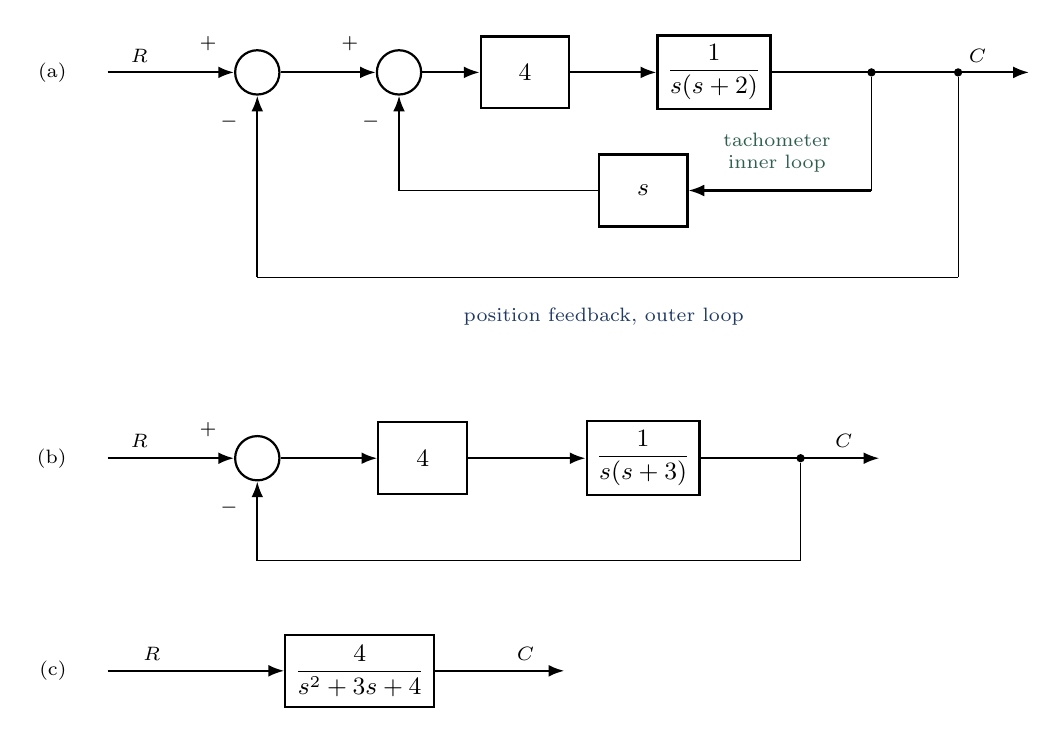
\begin{tikzpicture}[x=1cm,y=1cm,font=\small]
% ---- (a) original two-loop diagram ----
\begin{scope}[shift={(0,0)}]
\node[font=\scriptsize,left] at (-1.0,0) {(a)};
\node[sumnode] (S1) at (1.3,0) {};
\node[sumnode] (S2) at (3.1,0) {};
\node[block] (A) at (4.7,0) {$4$};
\node[block] (M) at (7.1,0) {$\dfrac{1}{s(s+2)}$};
\node[pickoff] (P1) at (9.1,0) {};
\node[pickoff] (P2) at (10.2,0) {};
\node[block] (TAC) at (6.2,-1.5) {$s$};
\draw[sig] (-0.6,0) -- node[above,font=\scriptsize,pos=0.25]{$R$} (S1);
\draw[sig] (S1) -- (S2);
\draw[sig] (S2) -- (A);
\draw[sig] (A) -- (M);
\draw[sig] (M) -- (11.1,0) node[above,font=\scriptsize,pos=0.8]{$C$};
% inner tacho loop from P1
\draw (P1) -- (9.1,-1.5); \draw[sig] (9.1,-1.5) -- (TAC);
\draw (TAC) -- (3.1,-1.5); \draw[sig] (3.1,-1.5) -- (S2);
% outer unity loop from P2
\draw (P2) -- (10.2,-2.6); \draw (10.2,-2.6) -- (1.3,-2.6);
\draw[sig] (1.3,-2.6) -- (S1);
\sumsign{S1}{150}{+}
\sumsign{S1}{240}{-}
\sumsign{S2}{150}{+}
\sumsign{S2}{240}{-}
\node[faccent,font=\scriptsize,align=center] at (7.9,-1.02) {tachometer\\inner loop};
\node[fnavy,font=\scriptsize] at (5.7,-3.1) {position feedback, outer loop};
\end{scope}
% ---- (b) after inner loop collapsed ----
\begin{scope}[shift={(0,-4.9)}]
\node[font=\scriptsize,left] at (-1.0,0) {(b)};
\node[sumnode] (T1) at (1.3,0) {};
\node[block] (B1) at (3.4,0) {$4$};
\node[block] (B2) at (6.2,0) {$\dfrac{1}{s(s+3)}$};
\node[pickoff] (Q) at (8.2,0) {};
\draw[sig] (-0.6,0) -- node[above,font=\scriptsize,pos=0.25]{$R$} (T1);
\draw[sig] (T1) -- (B1);
\draw[sig] (B1) -- (B2);
\draw[sig] (B2) -- (9.2,0) node[above,font=\scriptsize,pos=0.8]{$C$};
\draw (Q) -- (8.2,-1.3); \draw (8.2,-1.3) -- (1.3,-1.3);
\draw[sig] (1.3,-1.3) -- (T1);
\sumsign{T1}{150}{+}
\sumsign{T1}{240}{-}
\end{scope}
% ---- (c) final ----
\begin{scope}[shift={(0,-7.6)}]
\node[font=\scriptsize,left] at (-1.0,0) {(c)};
\node[block] (F) at (2.6,0) {$\dfrac{4}{s^{2}+3s+4}$};
\draw[sig] (-0.6,0) -- node[above,font=\scriptsize,pos=0.25]{$R$} (F);
\draw[sig] (F) -- (5.2,0) node[above,font=\scriptsize,pos=0.7]{$C$};
\end{scope}
\end{tikzpicture}
\caption{Worked example~4.2 reduced in stages: (a) the servo with tachometer
and position feedback, (b) after the inner loop is collapsed --- note the
motor pole moving from $-2$ to $-3$, (c) the single closed-loop block.}
\label{fig:servo-reduce}
\end{figure}

% --------------------------------------------------------------------
\section{When reduction gets awkward: overlapping loops}
\label{sec:overlap}

Worked example~4.2 was easy because its loops were \textbf{nested}: the inner
loop sat entirely inside the outer one, so collapsing it left a diagram of the
same shape. Loops can also \textbf{overlap} --- each containing part, but not
all, of the other --- and then no amount of collapsing helps, because there is
no innermost loop to start from. Figure~\ref{fig:overlap}(a) is the smallest
example, and it is the standard one in every textbook.

\begin{figure}[htbp]
\centering
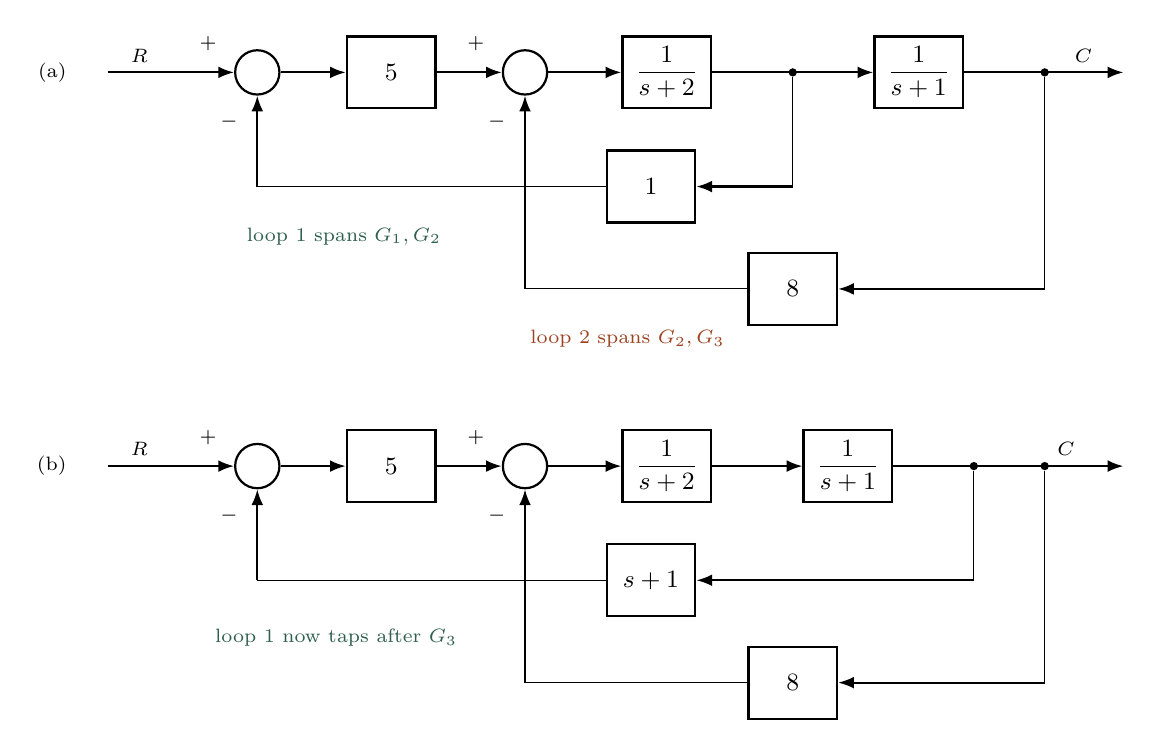
\begin{tikzpicture}[x=1cm,y=1cm,font=\small]
% ---- (a) overlapping loops ----
\begin{scope}[shift={(0,0)}]
\node[font=\scriptsize,left] at (-1.0,0) {(a)};
\node[sumnode] (S1) at (1.3,0) {};
\node[block] (G1) at (3.0,0) {$5$};
\node[sumnode] (S2) at (4.7,0) {};
\node[block] (G2) at (6.5,0) {$\dfrac{1}{s+2}$};
\node[pickoff] (P1) at (8.1,0) {};
\node[block] (G3) at (9.7,0) {$\dfrac{1}{s+1}$};
\node[pickoff] (P2) at (11.3,0) {};
\draw[sig] (-0.6,0) -- node[above,font=\scriptsize,pos=0.25]{$R$} (S1);
\draw[sig] (S1) -- (G1);
\draw[sig] (G1) -- (S2);
\draw[sig] (S2) -- (G2);
\draw[sig] (G2) -- (G3);
\draw[sig] (G3) -- (12.3,0) node[above,font=\scriptsize,pos=0.75]{$C$};
% loop 1: from P1 (output of G2) back to S1 through H1 = 1
\node[block] (H1) at (6.3,-1.45) {$1$};
\draw (P1) -- (8.1,-1.45); \draw[sig] (8.1,-1.45) -- (H1);
\draw (H1) -- (1.3,-1.45); \draw[sig] (1.3,-1.45) -- (S1);
% loop 2: from P2 (output of G3) back to S2 through H2 = 8
\node[block] (H2) at (8.1,-2.75) {$8$};
\draw (P2) -- (11.3,-2.75); \draw[sig] (11.3,-2.75) -- (H2);
\draw (H2) -- (4.7,-2.75); \draw[sig] (4.7,-2.75) -- (S2);
\sumsign{S1}{150}{+}
\sumsign{S1}{240}{-}
\sumsign{S2}{150}{+}
\sumsign{S2}{240}{-}
\node[faccent,font=\scriptsize] at (2.4,-2.08) {loop 1 spans $G_1,G_2$};
\node[fflag,font=\scriptsize] at (6.0,-3.38) {loop 2 spans $G_2,G_3$};
\end{scope}
% ---- (b) after moving the pick-off forward through G3 ----
\begin{scope}[shift={(0,-5.0)}]
\node[font=\scriptsize,left] at (-1.0,0) {(b)};
\node[sumnode] (T1) at (1.3,0) {};
\node[block] (F1) at (3.0,0) {$5$};
\node[sumnode] (T2) at (4.7,0) {};
\node[block] (F2) at (6.5,0) {$\dfrac{1}{s+2}$};
\node[block] (F3) at (8.8,0) {$\dfrac{1}{s+1}$};
\node[pickoff] (Q1) at (10.4,0) {};
\node[pickoff] (Q2) at (11.3,0) {};
\draw[sig] (-0.6,0) -- node[above,font=\scriptsize,pos=0.25]{$R$} (T1);
\draw[sig] (T1) -- (F1);
\draw[sig] (F1) -- (T2);
\draw[sig] (T2) -- (F2);
\draw[sig] (F2) -- (F3);
\draw[sig] (F3) -- (12.3,0) node[above,font=\scriptsize,pos=0.75]{$C$};
% moved loop 1: now taken after G3, so needs (s+1)
\node[block] (K1) at (6.3,-1.45) {$s+1$};
\draw (Q1) -- (10.4,-1.45); \draw[sig] (10.4,-1.45) -- (K1);
\draw (K1) -- (1.3,-1.45); \draw[sig] (1.3,-1.45) -- (T1);
% loop 2 unchanged
\node[block] (K2) at (8.1,-2.75) {$8$};
\draw (Q2) -- (11.3,-2.75); \draw[sig] (11.3,-2.75) -- (K2);
\draw (K2) -- (4.7,-2.75); \draw[sig] (4.7,-2.75) -- (T2);
\sumsign{T1}{150}{+}
\sumsign{T1}{240}{-}
\sumsign{T2}{150}{+}
\sumsign{T2}{240}{-}
\node[faccent,font=\scriptsize] at (2.3,-2.18) {loop 1 now taps after $G_3$};
\end{scope}
\end{tikzpicture}
\caption{Overlapping loops. In (a) neither loop contains the other, so there
is no inner loop to collapse first. In (b) the pick-off point of loop~1 has
been moved forward through $G_3$ --- its gain picking up a factor $s+1$ in
compensation --- which makes the two loops nested and the reduction routine.}
\label{fig:overlap}
\end{figure}

\begin{workedex}[breakable, title=Worked example 4.3 --- overlapping loops by block-diagram algebra]
For Figure~\ref{fig:overlap}(a), with
\[
  G_1=5,\qquad G_2=\frac{1}{s+2},\qquad G_3=\frac{1}{s+1},
  \qquad H_1=1,\qquad H_2=8,
\]
find $T(s)=C(s)/R(s)$.

\medskip
\textbf{Step 1 --- move the pick-off point.} Loop~1 is fed from the output of
$G_2$. Move that pick-off forward through $G_3$, compensating the branch with
$1/G_3=s+1$, as in Figure~\ref{fig:overlap}(b). Loop~1 now taps the same node
as loop~2, and loop~2 sits inside it: the loops are nested.

\medskip
\textbf{Step 2 --- collapse the inner loop} ($G_2G_3$ with $H_2$):
\[
  \frac{G_2G_3}{1+G_2G_3H_2}
  = \frac{\dfrac{1}{(s+1)(s+2)}}{1+\dfrac{8}{(s+1)(s+2)}}
  = \frac{1}{(s+1)(s+2)+8}
  = \frac{1}{s^{2}+3s+10} .
\]

\medskip
\textbf{Step 3 --- collapse the outer loop.} Its forward path is $G_1$ times
the result of step~2, and its feedback path is $H_1(s+1)=s+1$:
\[
  T(s)=\frac{\dfrac{5}{s^{2}+3s+10}}
            {1+\dfrac{5(s+1)}{s^{2}+3s+10}}
   =\frac{5}{s^{2}+3s+10+5s+5}
   =\frac{5}{s^{2}+8s+15}
   =\frac{5}{(s+3)(s+5)} .
\]

\medskip
\textbf{Check.} The d.c.\ gain is $T(0)=5/15=1/3$, and the closed-loop poles
are at $-3$ and $-5$: real, distinct and stable. Notice that the two open-loop
poles were at $-1$ and $-2$; feedback has again relocated them, this time
further into the left half plane.

\medskip
\textbf{The cost.} Getting here took a junction move, two loop collapses and a
redrawn diagram, and every one of those steps is a place to lose a factor. The
answer is right, but the method does not scale --- a diagram with three
overlapping loops would need several moves, and each redrawing invites error.
That is the problem \S\ref{sec:mason} solves.
\end{workedex}

% ====================================================================
\part*{Part B --- Signal flow graphs and Mason's gain formula}
\addcontentsline{toc}{part}{Part B}

% --------------------------------------------------------------------
\section{Signal flow graphs}
\label{sec:sfg}

A \textbf{signal flow graph} (SFG) carries exactly the same information as a
block diagram in a leaner notation, invented by S.~J.~Mason precisely so that
the reduction could be replaced by a formula.

\begin{itemize}[leftmargin=*]
\item A \textbf{node} is a signal. It is drawn as a small dot and labelled with
      the signal's name.
\item A \textbf{branch} is a directed line from one node to another, labelled
      with its gain. Travelling along it multiplies the signal by that gain.
\item The signal at any node is the \emph{sum} of everything arriving on the
      branches that end there.
\end{itemize}

That last rule is what removes the need for summing junctions: addition is
built into the meaning of a node, and a subtraction is carried by a branch of
gain $-H$ rather than a $-$ sign on a circle. Table~\ref{tab:dictionary}
is the translation, and Figure~\ref{fig:bd2sfg} shows it applied to the
canonical feedback form.

\begin{table}[htbp]
\centering
\caption{Block diagram and signal flow graph: the same content, two notations.}
\label{tab:dictionary}
\small
\renewcommand{\arraystretch}{1.25}
\begin{tabular}{@{}p{5.1cm}p{4.5cm}p{4.7cm}@{}}
\toprule
\textbf{Block diagram} & \textbf{Signal flow graph} & \textbf{Note}\\
\midrule
Block with transfer function $G$ & Branch of gain $G$ & The gain sits on the
line, not in a box\\
Signal on a connecting line & Node & Named signals become dots\\
Summing junction & Node (addition is implied) & Signs move onto the branch
gains\\
Pick-off point & Node with two or more outgoing branches & Each branch carries
the node's full value\\
Input (reference) & \textbf{Source node} --- only outgoing branches & Also
called an input node\\
Output (controlled variable) & \textbf{Sink node} --- only incoming branches &
Add a unit branch if the output node also feeds a loop\\
\bottomrule
\end{tabular}
\end{table}

\begin{figure}[htbp]
\centering
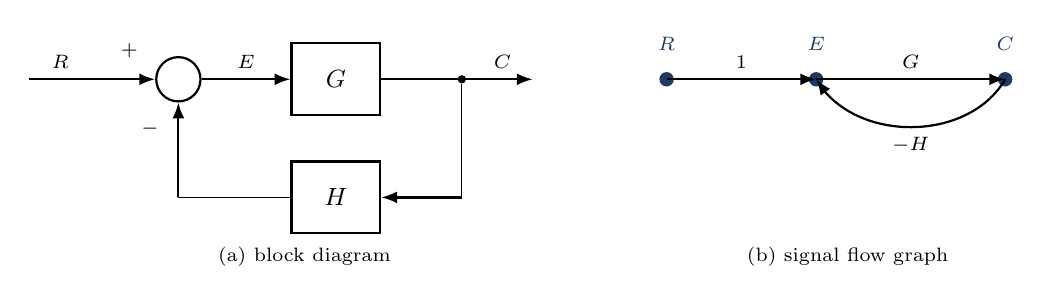
\begin{tikzpicture}[x=1cm,y=1cm,font=\small]
% ---- left: block diagram ----
\begin{scope}[shift={(0,0)}]
\node[sumnode] (S) at (1.4,0) {};
\node[block] (G) at (3.4,0) {$G$};
\node[pickoff] (P) at (5.0,0) {};
\node[block] (H) at (3.4,-1.5) {$H$};
\draw[sig] (-0.5,0) -- node[above,font=\scriptsize,pos=0.25]{$R$} (S);
\draw[sig] (S) -- node[above,font=\scriptsize]{$E$} (G);
\draw[sig] (G) -- (5.9,0) node[above,font=\scriptsize,pos=0.8]{$C$};
\draw (P) -- (5.0,-1.5); \draw[sig] (5.0,-1.5) -- (H);
\draw (H) -- (1.4,-1.5); \draw[sig] (1.4,-1.5) -- (S);
\sumsign{S}{150}{+}
\sumsign{S}{240}{-}
\node[font=\scriptsize] at (3.0,-2.25) {(a) block diagram};
\end{scope}
% ---- right: signal flow graph ----
\begin{scope}[shift={(7.6,0)}]
\foreach \x/\n/\lab in {0/R/$R$, 1.9/E/$E$, 4.3/C/$C$}{
  \fill[fnavy] (\x,0) circle (2.6pt);
  \node[fnavy,font=\scriptsize,above=7pt] at (\x,0) {\lab};}
\draw[sig] (0,0) -- node[above,font=\scriptsize,pos=0.5]{$1$} (1.9,0);
\draw[sig] (1.9,0) -- node[above,font=\scriptsize,pos=0.5]{$G$} (4.3,0);
% feedback branch, curved below
\draw[sig] (4.3,0) to[out=-120,in=-60] node[below,font=\scriptsize,pos=0.5]{$-H$} (1.9,0);
\node[font=\scriptsize] at (2.3,-2.25) {(b) signal flow graph};
\end{scope}
\end{tikzpicture}
\caption{The canonical feedback form in both notations. The summing junction
becomes the node $E$, and its minus sign is absorbed into the feedback branch
gain $-H$. Cf.\ Nise \S5.4, p.~248; Nagrath \& Gopal Fig.~2.25, p.~45.}
\label{fig:bd2sfg}
\end{figure}

The vocabulary Mason's formula needs is all about routes through the graph.
Figure~\ref{fig:sfgterms} is a graph carrying one of each.

\begin{itemize}[leftmargin=*]
\item A \textbf{path} is any route along branches, following the arrows, that
      passes through no node twice.
\item A \textbf{forward path} is a path from the source node to the sink node.
      Its \textbf{forward-path gain} is the product of the gains along it.
\item A \textbf{loop} is a closed path that starts and ends at the same node,
      visiting no other node twice. Its \textbf{loop gain} is the product of
      the gains around it --- including the minus signs.
\item Two loops are \textbf{non-touching} if they share \emph{no node at all}.
\end{itemize}

\begin{figure}[htbp]
\centering
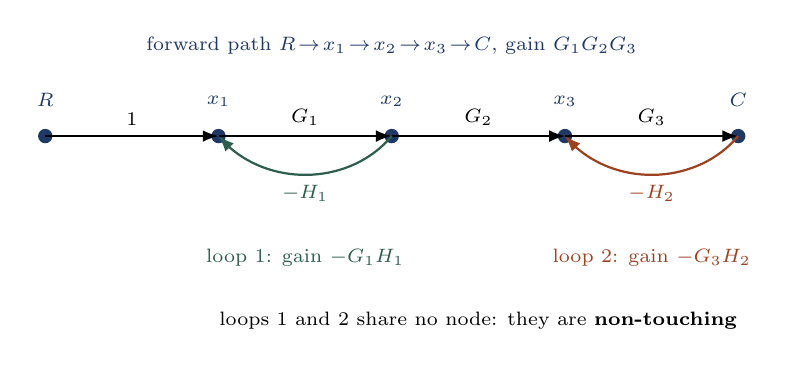
\begin{tikzpicture}[x=1cm,y=1cm,font=\small]
\foreach \x/\lab in {0/$R$, 2.2/$x_1$, 4.4/$x_2$, 6.6/$x_3$, 8.8/$C$}{
  \fill[fnavy] (\x,0) circle (2.6pt);
  \node[fnavy,font=\scriptsize,above=7pt] at (\x,0) {\lab};}
\draw[sig] (0,0) -- node[above,font=\scriptsize]{$1$} (2.2,0);
\draw[sig] (2.2,0) -- node[above,font=\scriptsize]{$G_1$} (4.4,0);
\draw[sig] (4.4,0) -- node[above,font=\scriptsize]{$G_2$} (6.6,0);
\draw[sig] (6.6,0) -- node[above,font=\scriptsize]{$G_3$} (8.8,0);
% loop A between x1 and x2
\draw[sig,faccent] (4.4,0) to[out=-130,in=-50] node[below,font=\scriptsize]{$-H_1$} (2.2,0);
% loop B between x3 and C
\draw[sig,fflag] (8.8,0) to[out=-130,in=-50] node[below,font=\scriptsize]{$-H_2$} (6.6,0);
% annotations
\node[faccent,font=\scriptsize,align=center] at (3.3,-1.55) {loop 1: gain $-G_1H_1$};
\node[fflag,font=\scriptsize,align=center] at (7.7,-1.55) {loop 2: gain $-G_3H_2$};
\node[fnavy,font=\scriptsize,align=center] at (4.4,1.15)
  {forward path $R\!\to\!x_1\!\to\!x_2\!\to\!x_3\!\to\!C$, gain $G_1G_2G_3$};
\node[font=\scriptsize,align=center] at (5.5,-2.35)
  {loops 1 and 2 share no node: they are \textbf{non-touching}};
\end{tikzpicture}
\caption{Signal flow graph vocabulary. Loop~1 touches nodes $x_1,x_2$ and
loop~2 touches $x_3,C$; because those sets are disjoint, the two loops are
non-touching, and Mason's formula will carry a product term for the pair.}
\label{fig:sfgterms}
\end{figure}

\begin{pitfall}
``Non-touching'' means \emph{no shared node} --- not ``drawn without
crossing'', and not ``no shared branch''. Two loops that meet at a single node
are touching, and contribute no product term. Getting this wrong is the most
common source of a wrong $\Delta$, and because the error is in a term you
simply failed to write, nothing in the algebra flags it. Check every pair of
loops explicitly: list each loop's nodes, then compare the lists.
\end{pitfall}

% --------------------------------------------------------------------
\section{Mason's gain formula}
\label{sec:mason}

Mason's gain formula reads the transfer function between a source node and a
sink node straight off the graph, with no redrawing at all:
\begin{equation}
  T(s) = \frac{\displaystyle\sum_{k} P_k\,\Delta_k}{\Delta} ,
  \label{eq:mason}
\end{equation}
where
\begin{itemize}[leftmargin=*]
\item $P_k$ is the gain of the $k$-th forward path, summed over \emph{all}
      forward paths;
\item $\Delta$ is the \textbf{determinant} of the graph, built from the loop
      gains as in \eqref{eq:delta} below;
\item $\Delta_k$ is the \textbf{cofactor} of path $k$: the determinant
      $\Delta$ recomputed with every loop that \emph{touches} path $k$ deleted
      from the graph.
\end{itemize}

\noindent
The determinant is an alternating sum over the loops, taken one at a time,
then in non-touching pairs, then in non-touching triples:
\begin{equation}
  \Delta = 1
    - \sum_{i} L_i
    + \sum_{\substack{\text{pairs }i,j\\ \text{non-touching}}} L_iL_j
    - \sum_{\substack{\text{triples }i,j,k\\ \text{non-touching}}} L_iL_jL_k
    + \cdots
  \label{eq:delta}
\end{equation}
where $L_i$ is the gain of the $i$-th loop, signs included. In this unit the
sum almost always stops at the pairs; triples need three loops that mutually
share no node, which takes a larger graph than any examination question here
will set.

Two special cases are worth noting before we use it. If every loop touches
every forward path --- which is true of most single-input single-output control
diagrams --- then every $\Delta_k=1$ and \eqref{eq:mason} collapses to
$\left(\sum_k P_k\right)/\Delta$. And for the canonical feedback form of
Figure~\ref{fig:bd2sfg}, there is one forward path $P_1=G$ and one loop
$-GH$, so $\Delta=1+GH$, $\Delta_1=1$, and Mason gives $T=G/(1+GH)$ --- the
formula of \S\ref{sec:connections}, recovered as the simplest possible case.

\begin{keyidea}
Block-diagram reduction and Mason's formula are two routes to the same
transfer function, and the choice between them is practical, not
mathematical. Reduction is clearer for a diagram with two or three nested
loops and tells a story about the physics as you go. Mason wins the moment
loops overlap or forward paths multiply, because it never requires the diagram
to be redrawn --- and a diagram that is never redrawn cannot be redrawn wrongly.
\end{keyidea}

\begin{workedex}[breakable, title={Worked example 4.4 --- the overlapping-loop system again, in one line}]
Take the system of Worked example~4.3 --- Figure~\ref{fig:overlap}(a), with
$G_1=5$, $G_2=1/(s+2)$, $G_3=1/(s+1)$, $H_1=1$, $H_2=8$ --- and apply Mason's
formula to it directly.

\medskip
\textbf{Forward paths.} There is one:
\[
  P_1 = G_1G_2G_3 = \frac{5}{(s+1)(s+2)} .
\]

\medskip
\textbf{Loops.} There are two. Loop~1 runs forward through $G_1$ and $G_2$ and
back through $H_1$; loop~2 runs forward through $G_2$ and $G_3$ and back
through $H_2$:
\[
  L_1 = -G_1G_2H_1 = -\frac{5}{s+2},
  \qquad
  L_2 = -G_2G_3H_2 = -\frac{8}{(s+1)(s+2)} .
\]
They both pass through the node at the output of $G_2$, so they
\emph{touch}: there is no non-touching pair, and $\Delta$ stops after the
loop-gain sum.

\medskip
\textbf{Determinant and cofactor.}
\[
  \Delta = 1-(L_1+L_2) = 1+\frac{5}{s+2}+\frac{8}{(s+1)(s+2)} ,
  \qquad \Delta_1 = 1
\]
($\Delta_1=1$ because the single forward path passes through both loops).

\medskip
\textbf{Result.} Multiplying numerator and denominator of \eqref{eq:mason} by
$(s+1)(s+2)$,
\[
  T(s)=\frac{P_1\Delta_1}{\Delta}
   =\frac{5}{(s+1)(s+2)+5(s+1)+8}
   =\frac{5}{s^{2}+8s+15}
   =\frac{5}{(s+3)(s+5)} ,
\]
which is exactly the answer Worked example~4.3 obtained --- with no pick-off
move, no redrawn diagram and no intermediate transfer functions to mislay.
\end{workedex}

\begin{workedex}[breakable, title={Worked example 4.5 --- two forward paths and a non-touching pair}]
Figure~\ref{fig:mason-ex} shows a graph with a feedforward branch and two
loops that do not touch. Take
\[
  G_1=1,\quad G_2=\frac{2}{s+1},\quad G_3=\frac{1}{s+2},\quad G_4=4,
  \quad G_5=2,\quad H_1=3,\quad H_2=2 .
\]
Find $T(s)=C(s)/R(s)$.

\medskip
\textbf{Forward paths.} Two:
\[
  P_1 = G_1G_2G_3G_4 = \frac{8}{(s+1)(s+2)}
  \qquad\text{(through the whole chain)},
\]
\[
  P_2 = G_5 = 2
  \qquad\text{(the feedforward branch $x_1\to C$)} .
\]

\medskip
\textbf{Loops.} Two: $L_1=-G_1H_1=-3$ around $x_1,x_2$, and
$L_2=-G_3H_2=-2/(s+2)$ around $x_3,x_4$. Their node sets
$\{x_1,x_2\}$ and $\{x_3,x_4\}$ are disjoint, so this pair \emph{is}
non-touching and contributes a product term:
\[
  \Delta = 1-(L_1+L_2)+L_1L_2
   = 1+3+\frac{2}{s+2}+\frac{6}{s+2}
   = 4+\frac{8}{s+2}
   = \frac{4(s+4)}{s+2} .
\]

\medskip
\textbf{Cofactors.} Path $P_1$ runs through every node of both loops, so
$\Delta_1=1$. Path $P_2$ leaves the chain at $x_1$, so it touches loop~1 but
\emph{not} loop~2 --- loop~2 survives in its cofactor:
\[
  \Delta_2 = 1 - L_2 = 1+\frac{2}{s+2}=\frac{s+4}{s+2} .
\]

\medskip
\textbf{Result.}
\[
  T(s)=\frac{P_1\Delta_1+P_2\Delta_2}{\Delta}
   =\frac{\dfrac{8}{(s+1)(s+2)}+\dfrac{2(s+4)}{s+2}}
         {\dfrac{4(s+4)}{s+2}} ,
\]
and multiplying numerator and denominator by $(s+1)(s+2)$,
\[
  T(s)=\frac{8+2(s+4)(s+1)}{4(s+4)(s+1)}
   =\frac{2s^{2}+10s+16}{4(s+1)(s+4)}
   =\frac{s^{2}+5s+8}{2(s+1)(s+4)} .
\]

\medskip
\textbf{Reading the answer.} The closed-loop poles are at $-1$ and $-4$, and
the d.c.\ gain is $T(0)=8/8=1$. The interesting part is the numerator: the
feedforward path has given the system a pair of \emph{zeros}, at
$s=-2.5\pm\mathrm{j}1.32$, where the chain alone had none. This is Week~3's
lesson arriving from a new direction --- a parallel route through a system
puts zeros in its transfer function, and those zeros reshape the transient
without changing a single pole.
\end{workedex}

\begin{figure}[htbp]
\centering
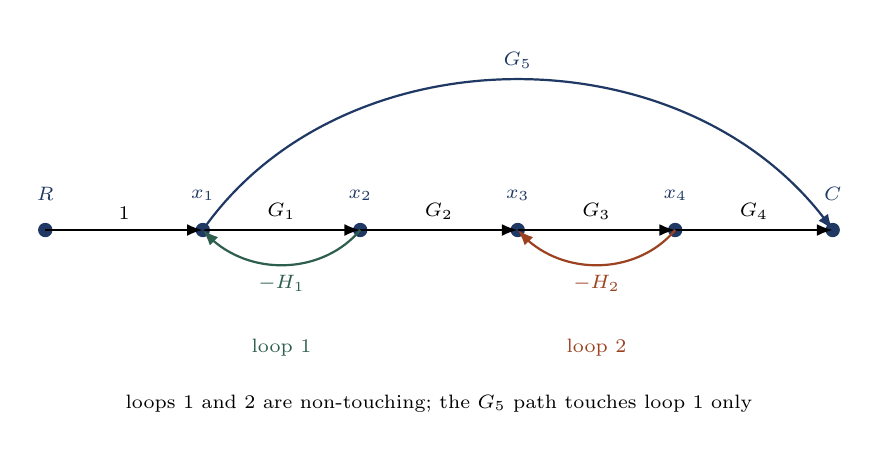
\begin{tikzpicture}[x=1cm,y=1cm,font=\small]
\foreach \x/\lab in {0/$R$, 2.0/$x_1$, 4.0/$x_2$, 6.0/$x_3$, 8.0/$x_4$, 10.0/$C$}{
  \fill[fnavy] (\x,0) circle (2.6pt);
  \node[fnavy,font=\scriptsize,above=7pt] at (\x,0) {\lab};}
\draw[sig] (0,0) -- node[above,font=\scriptsize]{$1$} (2.0,0);
\draw[sig] (2.0,0) -- node[above,font=\scriptsize]{$G_1$} (4.0,0);
\draw[sig] (4.0,0) -- node[above,font=\scriptsize]{$G_2$} (6.0,0);
\draw[sig] (6.0,0) -- node[above,font=\scriptsize]{$G_3$} (8.0,0);
\draw[sig] (8.0,0) -- node[above,font=\scriptsize]{$G_4$} (10.0,0);
% feedforward path x1 -> C, drawn well above the chain
\draw[sig,fnavy] (2.0,0) to[out=55,in=125] node[above,font=\scriptsize,pos=0.5]{$G_5$} (10.0,0);
% loop 1 (x1,x2)
\draw[sig,faccent] (4.0,0) to[out=-130,in=-50] node[below,font=\scriptsize]{$-H_1$} (2.0,0);
% loop 2 (x3,x4)
\draw[sig,fflag] (8.0,0) to[out=-130,in=-50] node[below,font=\scriptsize]{$-H_2$} (6.0,0);
\node[faccent,font=\scriptsize] at (3.0,-1.5) {loop 1};
\node[fflag,font=\scriptsize] at (7.0,-1.5) {loop 2};
\node[font=\scriptsize,align=center] at (5.0,-2.2)
  {loops 1 and 2 are non-touching; the $G_5$ path touches loop~1 only};
\end{tikzpicture}
\caption{Worked example~4.5: a graph with two forward paths (the chain, and
the feedforward branch $G_5$) and a non-touching pair of loops. Cf.\ Nise
\S5.5, p.~251.}
\label{fig:mason-ex}
\end{figure}

% --------------------------------------------------------------------
\section{Systems with more than one input}
\label{sec:twoinput}

An LTI system's response to several inputs acting at once is the sum of its
responses to each acting alone --- superposition, which holds precisely because
the system is linear. In block-diagram terms: to find the transfer function
from one input, set all the other inputs to zero and reduce the diagram as
usual; then add the contributions.

\begin{figure}[htbp]
\centering
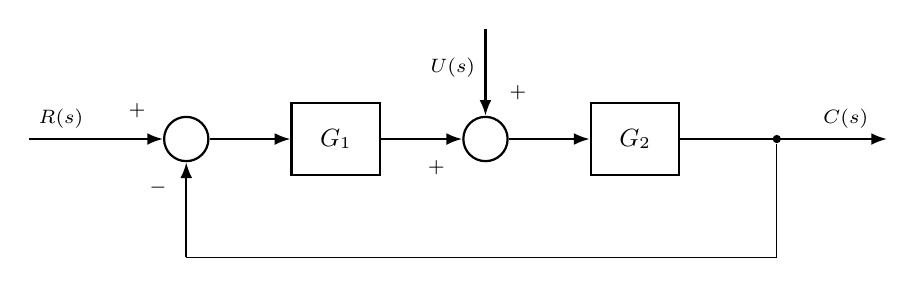
\begin{tikzpicture}[x=1cm,y=1cm,font=\small]
\node[sumnode] (S1) at (1.5,0) {};
\node[block] (G1) at (3.4,0) {$G_1$};
\node[sumnode] (S2) at (5.3,0) {};
\node[block] (G2) at (7.2,0) {$G_2$};
\node[pickoff] (P) at (9.0,0) {};
\draw[sig] (-0.5,0) -- node[above,font=\scriptsize,pos=0.24]{$R(s)$} (S1);
\draw[sig] (S1) -- (G1);
\draw[sig] (G1) -- (S2);
\draw[sig] (S2) -- (G2);
\draw[sig] (G2) -- (10.4,0) node[above,font=\scriptsize,pos=0.8]{$C(s)$};
\draw[sig] (5.3,1.4) -- node[left,font=\scriptsize,pos=0.45]{$U(s)$} (S2);
\draw (P) -- (9.0,-1.5); \draw (9.0,-1.5) -- (1.5,-1.5);
\draw[sig] (1.5,-1.5) -- (S1);
\sumsign{S1}{150}{+}
\sumsign{S1}{240}{-}
\sumsign{S2}{210}{+}
\sumsign{S2}{55}{+}
\end{tikzpicture}
\caption{A system with a second input $U$ entering between the two forward
blocks. Its response is found by superposition: one reduction with $U=0$, a
second with $R=0$.}
\label{fig:twoinput}
\end{figure}

Take Figure~\ref{fig:twoinput} with $G_1=2$, $G_2=3/(s+1)$ and unity feedback.
Setting $U=0$ leaves the canonical form with forward path $G_1G_2=6/(s+1)$:
\[
  \frac{C(s)}{R(s)} = \frac{G_1G_2}{1+G_1G_2}
   = \frac{\dfrac{6}{s+1}}{1+\dfrac{6}{s+1}}
   = \frac{6}{s+7} .
\]
Setting $R=0$ instead, $U$ sees only $G_2$ on the way out, but the same loop on
the way round:
\[
  \frac{C(s)}{U(s)} = \frac{G_2}{1+G_1G_2}
   = \frac{\dfrac{3}{s+1}}{1+\dfrac{6}{s+1}}
   = \frac{3}{s+7} ,
\]
and the total response is
\[
  C(s) = \frac{6}{s+7}R(s) + \frac{3}{s+7}U(s) .
\]
The two transfer functions share a denominator --- necessarily, since both are
governed by the same characteristic equation $1+G_1G_2=0$ --- and differ only
in numerator, because $U$ enters the loop further downstream and so is
amplified less. Here a unit step at $U$ produces half the steady-state output
of a unit step at $R$.

\begin{keyidea}
Superposition means one characteristic equation, several numerators. Extra
inputs change \emph{what} the system responds to; they cannot change
\emph{how} it responds, because the poles belong to the loop, not to the input.
\end{keyidea}

\noindent
\emph{Where this stops in FEE3411.} When the second input is something
unwanted --- a load torque, a supply fluctuation, sensor noise --- it is called
a disturbance, and the interesting question becomes how to design a loop that
rejects it. Computing the response, as above, is analysis and belongs here.
Designing for disturbance rejection, and dealing with plant uncertainty and
measurement noise, is FEE3412's work; Khalil \S4-4 to \S4-8 and Nise \S7.5 and
\S7.7 are worth reading for interest, but are not examinable in this unit.

% --------------------------------------------------------------------
\section*{Summary}

\begin{itemize}
\item A block diagram has three elements --- block, summing junction, pick-off
      point --- and encodes one algebraic equation in $s$ per block and per
      junction. A pick-off point copies a signal; it does not divide it.
\item Cascade gives $G_1G_2$, parallel gives $G_1\pm G_2$, negative feedback
      gives $G/(1+GH)$. The cascade rule assumes no loading between stages.
\item In canonical form, $G$ is the forward path, $GH$ the open-loop transfer
      function, $T=G/(1+GH)$ the closed-loop transfer function and
      $1/(1+GH)$ the error transfer function. The closed-loop poles are the
      roots of the characteristic equation $1+GH=0$.
\item Feedback does not change the number of poles; it relocates them. That
      relocation is the whole purpose of closing a loop.
\item Block-diagram algebra adds two moving rules: a summing junction moved
      against the flow divides by the block, and a pick-off point moved with
      the flow needs a compensating $1/G$ on the moved branch.
\item Nested loops reduce from the inside out. \emph{Overlapping} loops do not
      --- they need a junction move first, which is where hand reduction
      becomes error-prone.
\item A signal flow graph replaces blocks with branch gains and summing
      junctions with nodes, absorbing feedback signs into the branch gains.
\item Mason's gain formula, $T=\sum_kP_k\Delta_k/\Delta$, reads the transfer
      function off the graph with no redrawing. $\Delta$ alternates signs over
      loop gains, then products of non-touching pairs, then triples;
      $\Delta_k$ deletes the loops that touch path $k$. ``Non-touching'' means
      sharing no node.
\item Several inputs are handled by superposition: one transfer function per
      input, all sharing the same denominator.
\end{itemize}

% --------------------------------------------------------------------
\section*{Before the tutorial}

\begin{enumerate}
\item A unity-feedback system has $G(s)=12/[s(s+8)]$. Write down its open-loop
      transfer function, its characteristic equation, and its closed-loop
      transfer function. Are the closed-loop poles real or complex?
\item In the canonical form, which of $G$, $GH$ and $G/(1+GH)$ would a question
      mean by ``the loop gain''? Which sets the closed-loop poles?
\item A pick-off point sits before a block $G(s)=4/(s+3)$ and feeds a branch of
      gain $2$. Redraw it with the pick-off taken \emph{after} the block, and
      state the new branch gain.
\item Draw the signal flow graph of a unity-feedback system whose forward path
      is a cascade of $G_1$ and $G_2$, then use Mason's formula to confirm you
      get $G_1G_2/(1+G_1G_2)$. How many forward paths and loops did you find?
\end{enumerate}

% --------------------------------------------------------------------
\section*{Looking ahead}

This week finished the modelling half of FEE3411. From Week~2's differential
equations, through Week~3's transfer functions, to this week's interconnection
rules, we can now write down a single $T(s)$ for a complete control system ---
and every remaining week of the unit is about interrogating that one function.
Week~5 starts immediately: it takes the $\wn$ and $\zt$ read off denominators
like $s^{2}+3s+4$ in Worked example~4.2 and turns them into overshoot, rise
time, peak time and settling time. Week~6 asks what steady-state error the
response settles to, and Week~7 asks the question this week quietly set up ---
whether the roots of $1+G(s)H(s)=0$ are all in the left half plane at all.
Assignment~2, issued this week and due in Week~6, covers Weeks~3 and~4
together: transfer functions, block-diagram reduction, signal flow graphs and
Mason's rule. The boundary holds as always --- locating a closed-loop pole is
\emph{analysis} and belongs here; choosing $G(s)$ to put it somewhere better
is \emph{design}, and belongs to FEE3412.

\end{document}
